\label{sec:23}
\subsection{ARIMA modelling}
Using the "Penn World Tables v. 9.0"\footnote{Downloadable from \url{https://www.rug.nl/ggdc/productivity/pwt/}} I analyze the development in the logarithm of real GDP per capita (at 2011 national prices) from 1950-2014 for Spain, (Western) Germany, and Denmark\footnote{Before taking the log, the Danish Kroner (DKK) is transformed to Euros by multiplication with 7.46038 which is the central exchange rate at which the DKK is pegged to the Euro within a tiny 2.5\% band, according to the \href{https://en.wikipedia.org/wiki/European_Exchange_Rate_Mechanism}{European Exchange Rate Mechanism (ERM)}.}.
\\
\textbf{\textit{\begin{itemize}
  \item[a)] Plot the time series.
\end{itemize}}}\noindent
From figure \ref{fig:23a} below it is obvious that the series for actual values of log GDP are not stationary as should be expected while the transformed series might be. Therefore, we will work with these series of first-differences instead leading to not looking to model ARMA(p,q) models but ARIMA(p,1,q) models indicating the \nth{1} order transformation.
\begin{figure}[H]
  \caption{Time series and first differences of log real GDP per capita}
  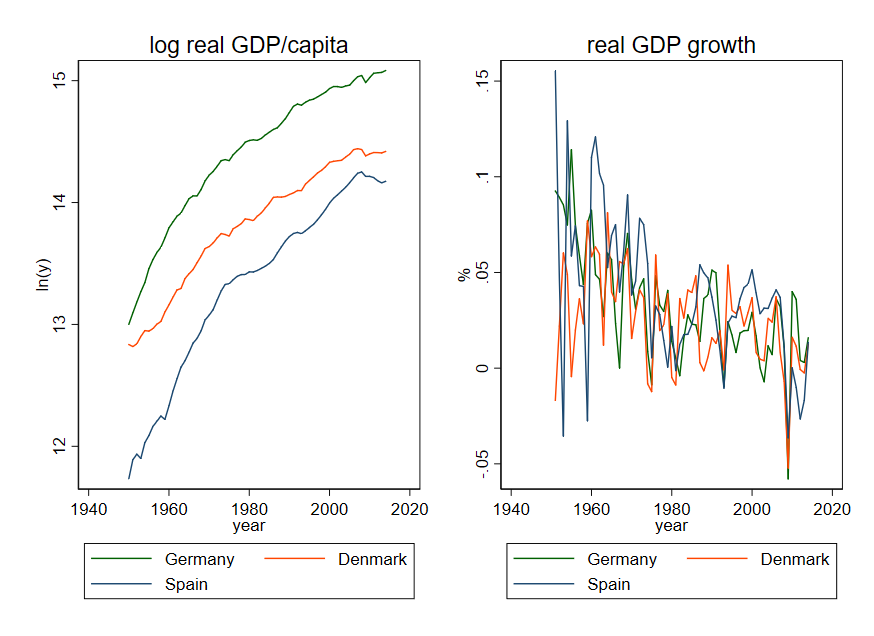
\includegraphics[width= \textwidth]{03_figures/fig23a}
  \label{fig:23a}
  \vspace{-1cm}
\end{figure}\noindent
However, the much higher growth rates in the 50s and 60s does raise the question of functional form even for the transformed processes of \nth{1} order. Is there a negative trend or a level shift? Also business cycles and especially negative shocks are evident. All three countries experience negative growth due to the global recessions in 1993 and 2009. Furthermore Denmark was hit significantly by the oil crisis in 1974-75 and Germany in 1975. Denmark also started the 80s with negative growth rates due to the global recession, while Germany again only experienced detraction for one year in 1982 and likewise briefly in 2003 and 2009. The financial crisis showed persistent negative growth in Denmark in 2008-2009 and 2012-2013 as in Spain with detraction through 2011-13. Germany had a single year with zero growth in 1967 and Denmark and Spain also experienced short recessions during the 50s like the 1959 reaction to the Stabilization Plan in Spain.
\\
\textbf{\textit{\begin{itemize}
  \item[b)] Identification: using autocorrelation and partial autocorrelation functions, identify the orders of the ARIMA model. Compute both the numerical and graphical autocorrelation functions (including confidence bands)
\end{itemize}}}\noindent
The Autocorrelation Functions (ACFs) and Partial Autocorrelation Functions (PACFs) in figure \ref{fig:23b} below show first of all that we do not need to worry about unit roots as none of the lags have an autocorrelation coefficient above $0.6$.
\begin{figure}[H]
  \caption{ACFs and PACFs of growth in real GDP per capita in Germany, Denmark, and Spain}
  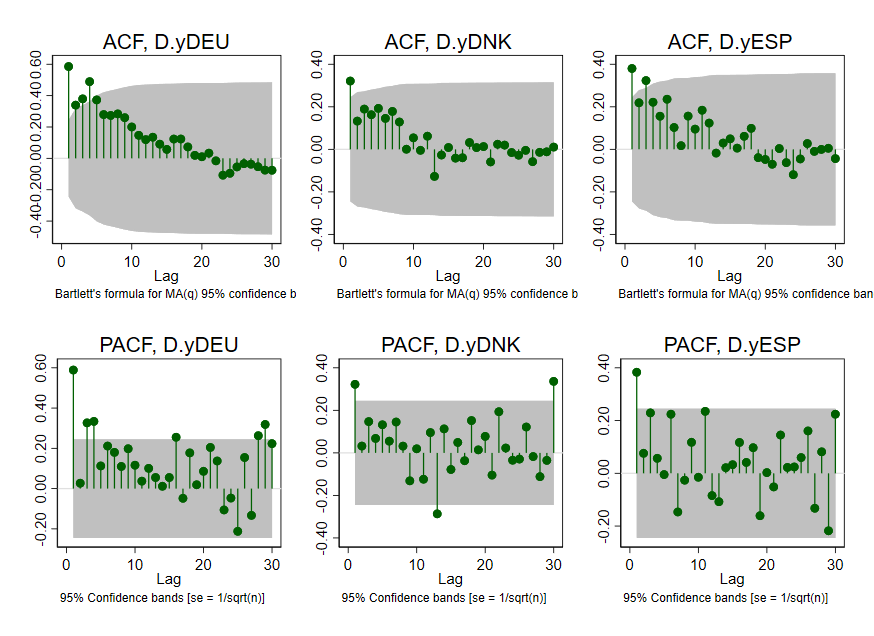
\includegraphics[width= \textwidth]{03_figures/fig23b}
  \label{fig:23b}
  \vspace{-1cm}
\end{figure}\noindent
The real GDP growth in Germany shows clear signs of autocorrelation for lags 1-4 and close to significant for autocorrelation for lag 5. In the partial autocorrelation function lag 1, 3-4, 16, and 28-30 are significant while 6-7 and 9 are close to significant. Computing the numerical correlogram Portmanteau's Q test for white noise clearly rejects that real GDP growth in Germany is a white noise process, on the contrary up to 30+ lags might be autocorrelated. The high number of lags in both the ACF and PACF suggests that German log real GDP per capita can be approximated by an ARIMA(p,1,q) model, that is, estimating growth in real GDP by an ARMA(p,q) model. While it is possible to estimate a model where only lag $q=1, 3,4, 16, 28,29,30$ are included, it is economically unrealistic and the later lags are obviously 'false signals' that can be due to model shifting caused by to structural breaks, e.g. the recessions in the German economy highlighted above. That aside, the graphical representation with the confidence bands is more consistent with up to 4 ACF lags and 4 PACF lags, thus initially suggesting an ARMA(4,4) model though different combinations of included lags $p\leq4$ and $q\leq4$ could be feasible as well.
\\
\\
While the graphical plots of both the ACF and PACF for real GDP growth in Denmark only show that the firsts lag are within the 95\% confidence several lags up to 7 gets close to the confidence bands and lag 13 is significantly autocorrelated with time $t$. Even more so the correlogram still show signs of autocorrelation and partial autocorrelation. In fact it is not until all the 12 first lags are included, that the Q test rejects the null-hypothesis that there at a 5\% significance level is no autocorrelation in the sample. This gives confidence that we can try an ARMA(1,1) model. Especially if controlling for some of the no less than 12 out of the 64 periods with negative growth in Denmark that might cause 'false signals'.

The stochastic process for Spain show less evidence of autocorrelation and partial autocorrelation than for Germany but a little more than for Denmark. We will likewise use an ARMA(1,1) model but also try out modeling growth in real GDP by an AR(1), AR(3), ARMA(3,3), ARMA(3,1), or ARMA(1,3) and test all four against each other, as lag 3 is about borderline significantly autocorrelated and partially autocorrelated as well.
\\
\\
For all three countries, however, the PACFs in figure \ref{fig:23b} seem very close to zero for lag 2 which could cause issues trying to estimate ARIMA(p,q) models of order $q>1$.
\\
\textbf{\textit{\begin{itemize}
  \item[c)] Estimation: fit the identified ARIMA specification, using MLE estimation procedures
\end{itemize}}}\noindent
The ACFs and PACFs in figure \ref{fig:23b} showed that for each country several different model specifications could be reasonable suggestions for modelling real GDP growth. Therefore, all of the more likely model specifications are estimated and compared both in terms of the within-sample fit according to the Information Criteria (IC) and on the realism of the model based on the significance of the estimated parameters according to the z test statistic.
\\
\\
For Germany the baseline ARMA(4,4) is tested against an ARMA(4,1) and ARMA(1,4) model. The latter clearly surpasses the first two in terms of both IC and due to the parameter estimates actually being significant besides from the parameters for lag $q=3,4$ that are insignificant for all. The ARMA(1,2) and the ARMA(2,2) model do not even converge (not surprisingly, keeping the PACF in figure \ref{fig:23b} in mind). Instead the ARMA(1,4) is instead tested against the ARMA(1,1), AR(1) and MA(1) model. As the Akaike Information Criterion (AIC) points towards the ARMA(1,4) while the Bayesian IC (BIC) points towards the ARMA(1,1) specification we still have a subjective choice to make.

In the spirit of Milton Friedman's methodology of positive economics we could go with the ARIMA(1,1,4) model in order to maximize predictive power at the cost of using a less realistic model specification including insignificant parameters, especially $\hat{\theta}_3\sim0$ related to $q=3$. Oppositely we could follow the Parsimonious principle of estimating the more simple model in the ARMA(1,1). Though we should be well-knowing about the lost information from not including lag 3 and 4 that showed signs of significant in the PACF in figure \ref{fig:23b}.

All of the estimated ARMA(p,q) models have an estimate of the \nth{1} order autoregressive parameter $\hat{\phi}_1$ that is not significantly different from unity. Thus, only the persistence of shocks from the moving average elements prevents the model from acting as a random walk. An alternative further step would be to consider the AR(1) model that performs almost as good as the ARMA models and much better than the MA(1) model but with $\hat{\phi}_1=.62$ being far from unit root. In this autoregressive process there would only be indirect persistence of shocks, though. We will continue investigating the performance and implications of each of the three models throughout and the Maximum Likelihood (ML) estimates are shown in column (1)-(3) of table \ref{tab:23d}.
\\
\\
Table \ref{tab:23c} contain the estimates of the three models I choose to proceed with for Denmark and Spain. For Denmark the AR(1) model is clearly preferred as it has a lower AIC and BIC than both the ARMA(1,1) and the MA(1) that would be the two other reasonable specifications following the ACF and PACF in figure \ref{fig:23b}.
\begin{table}[H]
  \centering
  \caption{Estimates of ARMA models for growth in real GDP per capita in Denmark and Spain}
  \footnotesize
    \begin{tabular}{lccc}\toprule
            &(1) Denmark, AR(1)   &(2) Spain, ARMA(1,1)   &(3) Spain, AR(1)   \\
            &        b/se   &        b/se   &        b/se   \\
\midrule
cons       &       0.024***&       0.038   &       0.039***\\
            &     (0.004)   &     (0.024)   &     (0.008)   \\
\midrule
ARMA        &               &               &               \\
L.ar        &       0.332***&       0.923***&       0.443***\\
            &     (0.123)   &     (0.117)   &     (0.087)   \\
L.ma        &               &      -0.688***&               \\
            &               &     (0.164)   &               \\
\midrule
sigma       &       0.023***&       0.034***&       0.034***\\
            &     (0.002)   &     (0.002)   &     (0.002)   \\
\midrule
aic         &      -292.6   &      -244.5   &      -243.4   \\
bic         &      -286.1   &      -235.8   &      -236.9   \\
\bottomrule \end{tabular} \\ \text{Standard errors are in parentheses. * p<0.10, ** p<0.05, *** p<0.01}

  \label{tab:23c}
\end{table}\noindent
For Spain none of the models including $p=3$ or $q=3$ perform well, so the two preferred models are the ARMA(1,1) model with the lowest AIC and the AR(1) model with the lowest BIC. As for Germany it is not significant that $\hat{\phi}_1\neq1$ for the ARMA(1,1) model but it is for the AR(1) model.

\textbf{\textit{\begin{itemize}
  \item[d)] Validation: check the estimated residuals for misspecification errors
\end{itemize}}}\noindent
The residuals are computed and investigated for the estimated models. For Germany graphs for both the time series of the residuals, and their Autocorrelation Functions (ACFs) and Partial Autocorrelation Functions (PACFs) are shown in figure \ref{fig:residuals_dummies} in the appendix. First looking at the ARMA(1,4) none of the lags in the ACF for the residuals are significant. In the PACF only lag 15, 22, 25 are significant but it would not make sense to include these as lags of q in the ARMA(1,q). Thus, they must be so-called 'false signals' which could be explained by model shifting due to one of the structural breaks that we found earlier. The more sizable negative residuals are for the 2009-crisis followed by the 1974-75 oil-crisis and the 1993-recession. For the residuals of the ARMA(1,1) model the AC and PAC of lag 2 is significant, however, we know that the model does not converge when $q=2$ and that $\phi_2$ is not significant in an ARMA(2,1) model. The Q test is rejected for lags 2-6 meaning that they might be autocorrelated or partially autocorrelated That is, there is something left to be explained in the residuals and the model might be misspecified. For the AR(1) lag 4 of the residuals is significant and lag 2 close to significant for both the ACF and PACF the Q test is likewise rejected for lag 4.

Some of the stronger burst and busts might have disproportionately big impact on the size of the estimates and explain the mixed signals in the PACFs. Thus to improve the estimated models time dummies are included for the stronger structural breaks. To create a common criteria time dummies are included if the residual is 1.5 times bigger than the estimated standard error of the model $\hat{\sigma}$.\footnote{For the AR(1) model the same year dummies are included as for the ARMA(1,1) model since the standard error $\hat{\sigma}$ is relative high such that 2009 otherwise would be the only included negative outlier.} Table \ref{tab:23d} show the estimates of the ARMA(1,4), ARMA(1,1), and AR(1) models both with and without the inclusion of time dummies. Column 1-3 show the original models and column 4-6 show the same models but including time dummies for major structural breaks. The different models are compared to each other in terms of Information Criteria (IC) and simply by size and significance of the estimates. As expected both IC improve when controlling for 'outliers'. However the MA coefficients become highly insignificant for the ARIMA(1,1,4) where the standard errors explode to unacceptable dimensions for $q=1,4$ and $\hat{\theta}=1$ (column 4). Though still significant at a 5\% level the sign of $\hat{\theta}_1$ changes from negative to positive for the ARMA(1,1) model (column 5), an improvement however is that $\hat{\phi}_1$ is now significantly different from unity.
  \begin{table}[H]
    \centering
    \caption{Estimation of ARMA models for growth in real GDP per capita in Germany}
      \begin{tabular}{lcccccc}\toprule
            &(1) ARMA(1,4)   &(2) ARMA(1,1)   &   (3) AR(1)   &(4) ARMA(1,4)   &(5) ARMA(1,1)   &   (6) AR(1)   \\
            &        b/se   &        b/se   &        b/se   &        b/se   &        b/se   &        b/se   \\
\midrule
D.a51       &               &               &               &       0.001   &       0.005   &       0.002   \\
            &               &               &               &     (0.015)   &     (0.007)   &     (0.010)   \\
D.a55       &               &               &               &       0.023***&       0.019***&       0.017** \\
            &               &               &               &     (0.008)   &     (0.006)   &     (0.007)   \\
D.a63       &               &               &               &      -0.007*  &      -0.013** &      -0.015   \\
            &               &               &               &     (0.004)   &     (0.007)   &     (0.016)   \\
D.a74       &               &               &               &      -0.025***&      -0.014   &      -0.013   \\
            &               &               &               &     (0.004)   &     (0.009)   &     (0.008)   \\
D.a75       &               &               &               &      -0.044***&      -0.030** &      -0.033** \\
            &               &               &               &     (0.005)   &     (0.013)   &     (0.015)   \\
D.a93       &               &               &               &      -0.014***&      -0.014   &      -0.017   \\
            &               &               &               &     (0.004)   &     (0.017)   &     (0.013)   \\
D.a09       &               &               &               &      -0.045** &      -0.064***&      -0.066***\\
            &               &               &               &     (0.020)   &     (0.020)   &     (0.021)   \\
D.a10       &               &               &               &      -0.020   &      -0.030*  &      -0.031   \\
            &               &               &               &     (0.018)   &     (0.018)   &     (0.022)   \\
D.a67       &               &               &               &               &      -0.012***&      -0.018***\\
            &               &               &               &               &     (0.004)   &     (0.006)   \\
cons       &       0.043*  &       0.042*  &       0.034***&       0.042   &       0.034***&       0.035***\\
            &     (0.023)   &     (0.024)   &     (0.007)   &     (0.030)   &     (0.009)   &     (0.012)   \\
\midrule
ARMA        &               &               &               &               &               &               \\
L.ar        &       0.970***&       0.980***&       0.620***&       0.986***&       0.691***&       0.840***\\
            &     (0.044)   &     (0.031)   &     (0.073)   &     (0.030)   &     (0.131)   &     (0.085)   \\
L.ma        &      -0.535***&      -0.731***&               &      -0.665   &       0.410** &               \\
            &     (0.148)   &     (0.096)   &               &         (.)   &     (0.162)   &               \\
L2.ma       &      -0.384** &               &               &      -1.272***&               &               \\
            &     (0.175)   &               &               &     (0.149)   &               &               \\
L3.ma       &       0.021   &               &               &      -0.665***&               &               \\
            &     (0.175)   &               &               &     (0.232)   &               &               \\
L4.ma       &       0.294*  &               &               &       1.000   &               &               \\
            &     (0.155)   &               &               &         (.)   &               &               \\
\midrule
sigma       &       0.020***&       0.022***&       0.023***&       0.008***&       0.015***&       0.015***\\
            &     (0.002)   &     (0.002)   &     (0.002)   &     (0.001)   &     (0.002)   &     (0.002)   \\
\midrule
aic         &      -301.9   &      -297.0   &      -293.3   &      -342.5   &      -331.3   &      -330.7   \\
bic         &      -286.8   &      -288.4   &      -286.8   &      -314.4   &      -303.2   &      -304.8   \\
\bottomrule \end{tabular} \\ \text{Standard errors are in parentheses. * p<0.10, ** p<0.05, *** p<0.01}

    \label{tab:23d}
  \end{table}\noindent
As both estimated ARMA models seem to be quite unrobust to the ex- or inclusion of time dummies, this at first could seem to be where the AR(1) model comes to its right (column 6). The value of $\hat{phi}_1$ increases with the inclusion of time controls which is to be expected as it would need to undershoot before to not be too vulnerable to burst and busts. When including dummies both IC are lowest for the ARMA(1,4) model. When comparing the ARMA(1,1) and the AR(1) they are about level where the AIC is lower for the ARMA(1,1) and the BIC is lower for the AR(1) model.

While the IC naturally has improved a lot by removing some of the unexplained extremes, figure \ref{fig:residuals_dummies} in the appendix show that the ACFs, PACFs and the Q test for the residuals have only improved minimally. Nonetheless, f-or the ARMA(1,1) model it is just enough so that the Q test of no-autocorrelation of the residuals cannot be rejected for any lags. For the AR(1) without time dummies the Q test of the residuals was rejected for the \nth{4} lag that was also significant in both the ACF and the PACF. Including the time dummies have actually made the lag 2 of the residuals significant instead and now the Q test is rejected for lags 5-7. Clearly there is something left unexplained for the model, even with inclusion of time dummies. Therefore we reject the AR(1) model for Germany as misspecified and continue with the two ARMA models only.
\\
\\
For Denmark and Spain none of the lags of the residuals are significantly autocorrelated except for a few pointless partial autocorrelations of high-order lags as shown in figure \ref{fig:23d}. This is confirmed as none of the Q tests of no-autocorrelation in the residuals can be rejected. Thus, there is nothing left to be explained and our models seem well-specified. Yet it should be kept in mind that the autocorrelation and partial autocorrelation of the residuals in the AR(1) model for Spain are about borderline significantly for both lag 3 and 6 however which might possibly change if controlling for structural breaks as done for Germany.
\begin{figure}[H]
    \centering
    \caption{Residuals from modelling growth in real GDP per capita in Denmark and Spain}
      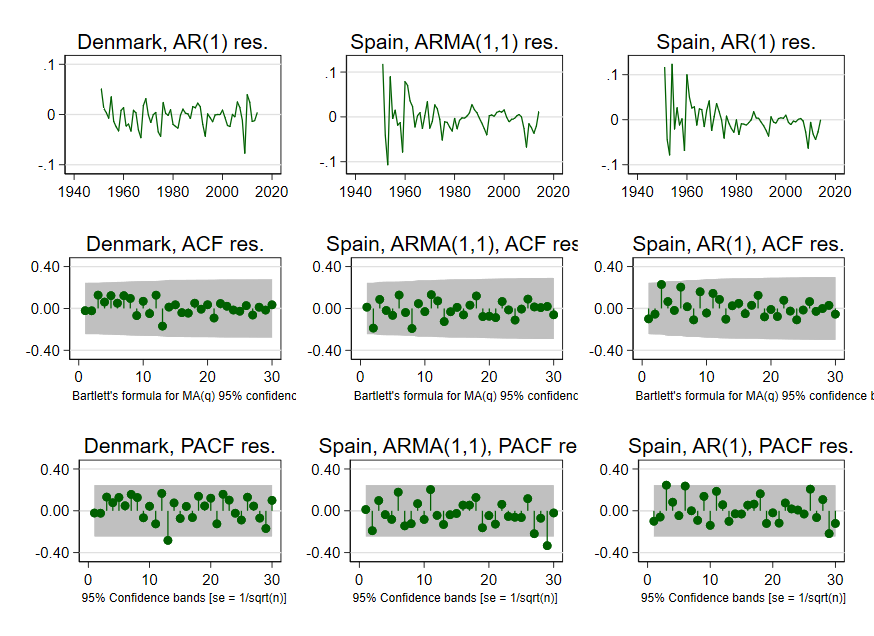
\includegraphics[width= \textwidth]{03_figures/fig23d}
    \label{fig:23d}
    \vspace{-2cm}
\end{figure}
\textbf{\textit{\begin{itemize}
    \item[e)] Forecasting: compute the one-step ahead forecast of the log of real GDP per capita time series
\end{itemize}}}\noindent
For Stata to be able to forecast even one-step ahead out of sample requires that the time dummies are set to zero, thus handling all of the sample as 'unknown' by disregarding beforehand-knowledge of which years will be extremes. The predictions of the growth rate in real GDP per capita in Germany of for each of the different models are shown in table \ref{tab:pred1}. It becomes very clear that while including dummies a model will certainly improve in terms of the within-sample fit, but the out-of-sample performance is definitely not guaranteed to improve. For the two ARMA models estimated without use of time dummies the prediction is a growth rate of 1.4\% for 2015 which is 0.2 percentage points less than the growth rate for 2014 in the sample. Reality has proven that the growth rate actually fell with exactly 0.2 percentage points.

The ARMA(1,1) model estimated using time dummies on the other hand predicts the growth rate to be a full percentage point higher. This reveals the nature of using time dummies for the estimation. As seen by the size and even the directions of the parameters in table \ref{tab:23d} the cautions in the predictions are removed when ignoring extreme observations by regarding them as exogenous shocks that will point the autoregressive process in another direction when needed, instead of regarding burst and busts endogenous phenomena that should be regarded as part of the process an estimated model should aim at capturing to some degree.

The forecast of negative growth of no less than 5.5\% by the ARMA(1,4) model estimated using times dummies is the direct results of the extreme values of the Moving Average terms where $\hat{\theta_2}=-1.3$ and $\hat{\theta_2}=1.0$. In fact these parameter values show that I for model selection probably should have been putting more emphasize on the features of the actual estimated parameters and be putting less weight on the IC and whether there were signs of autocorrelation in the residuals.
\begin{table}[H]
  \centering
  \caption{Predictions for 2015 growth in real GDP per capita, Germany}
    \begin{tabular}{lcccc}\toprule
            &\multicolumn{4}{c}{}                               \\
            & DyDEU\_pred1& DyDEU\_pred2& DyDEU\_pred3& DyDEU\_pred4\\
\midrule\\ Model&ARMA(1,4)&ARMA(1,1)&ARMA(1,4)&ARMA(1,1)\\ Time dummies&no&no&yes&yes\\ \midrule
mean        &        1.42&        1.40&       -5.52&        2.36\\
\bottomrule \end{tabular}

  \label{tab:pred1}
\end{table}
The AR(1) models predicts the growth in real GDP per capita for 2015 to be 2.0\% for Denmark and for 2.8\% for Spain. However the forecast of the ARMA(1,1) for Spain is more conservative at 0.7\%. For both countries the 2014 growth rate was around 1.3\% with negative growth rates in the years before that. Like the ARMA(1,1) model estimated without time dummies for Germany, the MA term $\hat{\theta}_1<0$ which is a mean reversion mechanism to correct for shocks. That is, going from negative growth rates in the previous years to a positive growth rate in 2014 implies very sizable positive residual which leads to the ARMA(1,1) prediction that the growth rate for Spain will drop significantly in 2015 as such a big residual should not be expected in the subsequent year as well. For 2015 this turned out to be untrue however, as the growth rate in Spain sky-rocketed to 3,4\% according to the World Bank.
\begin{table}[H]
  \centering
  \caption{Predictions for 2015 growth in real GDP per capita, Denmark and Spain}
  \footnotesize
    \begin{tabular}{lccc}\toprule
            &\multicolumn{3}{c}{}                  \\
            &  DyDNK\_pred& DyESP\_pred1&  DyESP\_pred\\
\midrule\\ Country&Denmark&Spain&Spain\\ Model&AR(1)&ARMA(1,1)&AR(1)\\ Time dummies&no&no&no\\ \midrule
mean        &        2.04&        0.71&        2.79\\
\bottomrule \end{tabular}

  \label{tab:pred2}
\end{table}

\textbf{\textit{\begin{itemize}
    \item[f)] Plot both the actual and predicted time series for each country
\end{itemize}}}\noindent
Figure \ref{fig:23f1}, \ref{fig:23f2}, and \ref{fig:23f3} performs visual evaluations of the predictive power 'out-of-sample' of each models by plotting the values that each model would predict year-by-year against the actual values. Furthermore, growth in real GDP per capita is forecasted the coming 10 years to see the inner workings of the models in the absence of new shocks.

Figure \ref{fig:23f1} evaluate the different models for Germany. While including year dummies for negative chocks clearly increases within-sample predictability, the downfall becomes very evident when predicting out of sample as well. The first panel show the predictions of the ARMA(1,4) model estimated with and without time dummies. The predictions of the dummy-model initially do a better job at capturing the full size of the fluctuations but then it seems that the oil-crisis of 1974-75, that is no longer controlled for, sparks a wild fluctuation where the model alternates between very excessive extremes. In panel two of \ref{fig:23f1} the ARMA(1,1) model estimated using dummies does a much better job. As seen in table \ref{tab:23d} the estimate of $\hat{\theta_1}$ becomes positive as time dummies prevents the model from over-shooting too much within-sample. However, out-of-sample the model basically acts as a linear extrapolation of the tendency in the period before, thus consistently 'overshoots' and fails to predict when business cycles turn. On the contrary the considerable size of the negative parameter $\hat{\theta_1}$ in the ARMA(1,1) model estimated without dummies overpredicts the mean-reversion to a degree where it almost does not capture any fluctuations but mostly corrects for, namely, a moving average of the time series.

The ARMA(1,1) model estimated using time dummies predicts that the growth rate in real GDP per capita converges towards no less than 3.4\& in 2014. While the trends of convergence are much more modest for the without-dummy estimations. The ARMA(1.4) and ARMA(1,1) models predict the growth rate in 2024 to be 2.0 and 1.9 respectively. This unrealistic level of optimism in the forecast is the result of both removing negative shocks from the training-sample of the model but also thereby reducing persistence of slumps.
\begin{figure}[H]
  \caption{Actual vs predicted growth in real GDP per capita, Germany}
  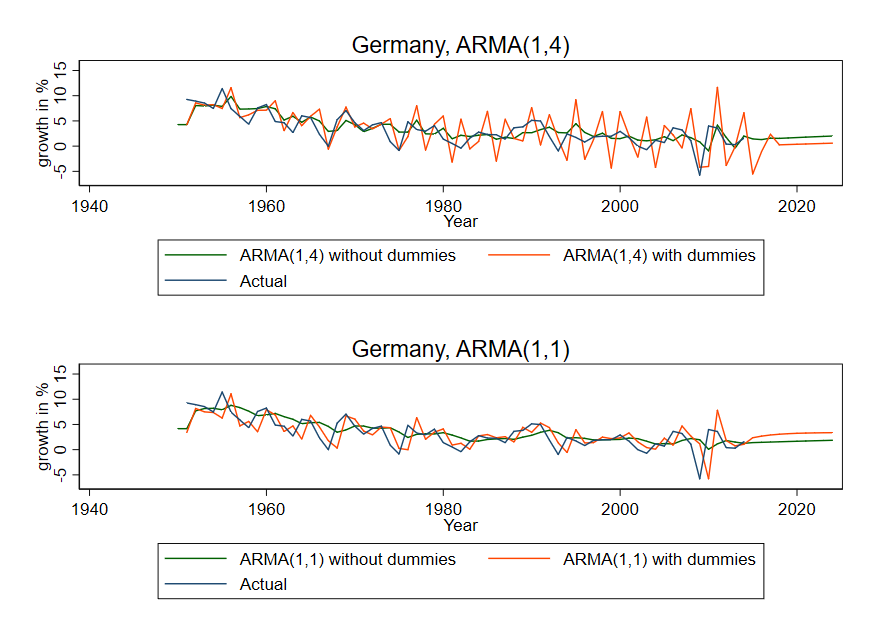
\includegraphics[width= \textwidth]{03_figures/fig23f1}
  \label{fig:23f1}
  \vspace{-1cm}
\end{figure}
It is clear that it is preferable not to use time dummies, at least not as extensively but only for an event that actually with high confidence is not expected to happen in a similar magnitude ever again. When deciding between the ARMA(1,4) and the ARMA(1,1) models both estimated without dummies, the choice in the end becomes subjective and depends on which qualities are appreciated as seen in figure \ref{fig:23f2} below. Recalling table \ref{tab:23d} the ARMA(1,4) has the lower value of the AIC as she model better fits the magnitude of business cycles when guessing right. On the downside, the size of wrong predictions and overshooting are more extreme as well. Literally and figuratively the predictive power of the ARMA(1,1) has both higher highs and lower lows. As an example, for 1995 the optimistic forecast was that the growth rate would go up by 1.8 percentage points. Instead it fell by 0.7 percentage points. Such a sizable prediction error could put an institution in a bad light. Thus, an economist that does not want to run such a risk could instead take the more cautious approach of leaning more towards the BIC that points towards the ARMA(1,1) model. This is reflected in the variance of the predicted time series being much smaller than for the actual time series. However, the model looses relevance if it at a too high degree just becomes an indication of the average of the growth rate in the recent years.
\begin{figure}[H]
  \caption{Actual vs predicted growth in real GDP, Germany}
  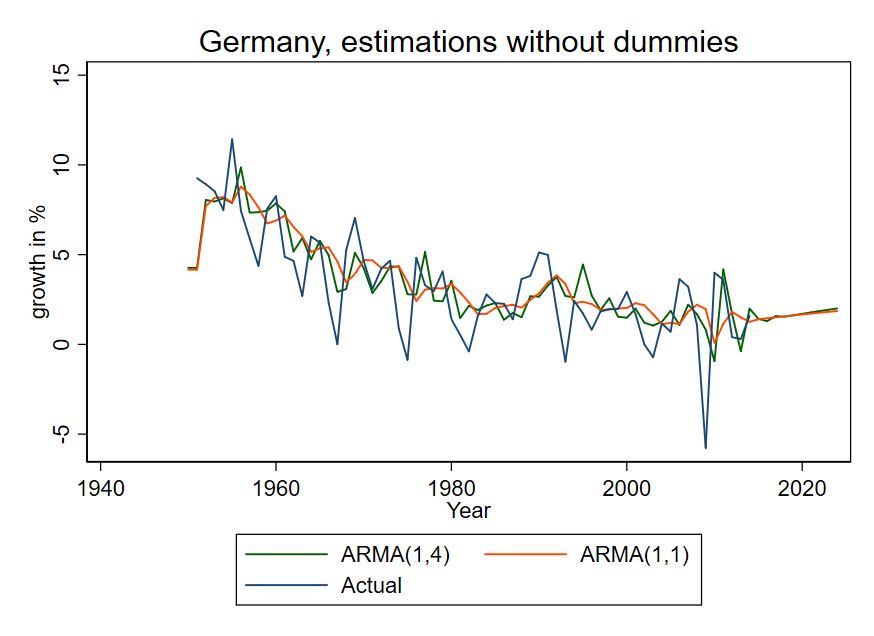
\includegraphics[width= \textwidth]{03_figures/fig23f2}
  \label{fig:23f2}
  \vspace{-1cm}
\end{figure}
In figure \ref{fig:23f3} for Denmark and Spain we see that the ARMA(1,1) model for Spain naturally only does a moderately good job at predicting when a boom or bust will end. But even more so, the AR(1) model for both Denmark and Spain has the mechanic of simply extrapolating the growth rate in the former period. Both model types will cause prediction error whenever a business cycle turns which leads to smaller parameter sizes to reduce the size of these prediction errors weighted against the cost of deliberately undershooting when, after all, predicting the right direction for most of the periods.
\begin{figure}[H]
  \caption{Actual vs predicted growth in real GDP per capita, Denmark and Spain}
  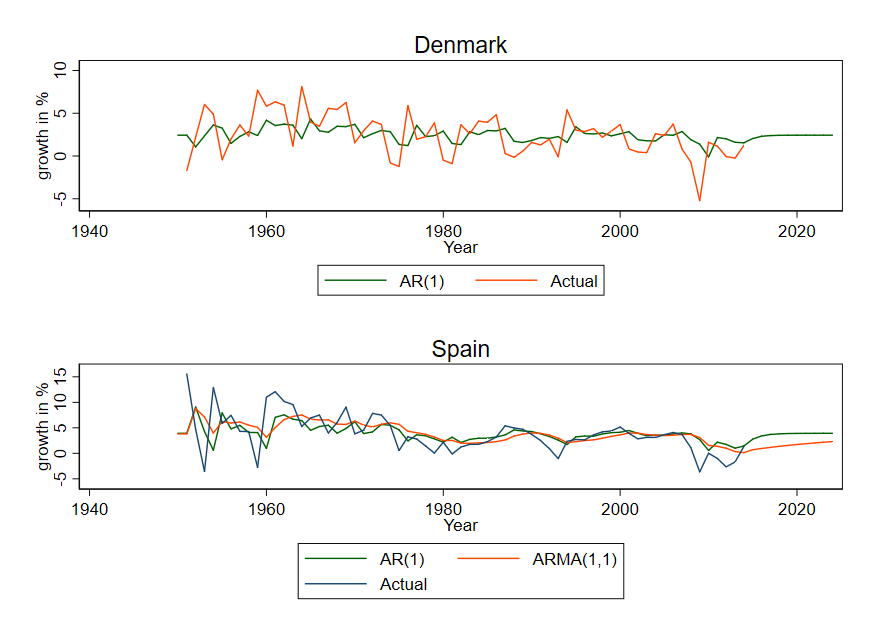
\includegraphics[width= \textwidth]{03_figures/fig23f3}
  \label{fig:23f3}
  \vspace{-1cm}
\end{figure}
